\chapter{Assessment of Renal $T_2$ Mapping Methods}
\label{chap:t2_mapping}

\begin{abstract}
	This work was presented as an aural presentation at the \ac{ISMRM} 28th Annual Meeting (2020) \cite{daniel_comparison_2020}.
	
	\lipsum[1]
\end{abstract}
\newpage
\acresetall

\section{Introduction}
\label{sec:t2_intro}
Quantitative \ac{MRI} is the process of taking measurements where the voxel values have numerical significance rather than simply representing signal intensity in arbitrary units \cite{tofts_quantitative_2003}. These numerically significant values can take the form of macroscale properties such as rate of oxygen consumption and blood vessel flow rates or microscale properties such as tissue \tone and susceptibility. When interpreted these values can be used improve diagnostic and treatment of patients.

The kidneys are structurally and functionally complex organs and as such lend themselves to the wide variety of MRI protocols designed to probe different aspects of the tissue and processes carried out within. While high resolution images of the kidneys morphology and basic measures such as \ac{TKV} can be very useful in diagnosing and monitoring disease progression \cite{buchanan_quantitative_2019, chapman_kidney_2012, gong_relationship_2012}, these do not fully leverage the quantitative nature of \ac{MRI}. Measurements of \tone have been shown to correlate well with fibrosis in the myocardium \cite{bull_human_2013, ferreira_t1_2013}, liver \cite{hoad_study_2015, luetkens_quantification_2018} and kidneys \cite{friedli_new_2016} and more generally an increase in \tone is associated with \ac{CKD} \cite{gillis_non-contrast_2016, cox_multiparametric_2017, buchanan_quantitative_2019}. \ac{ASL} techniques can be used to quantify renal perfusion in physiological units (mL/100g/min) and has been shown to be correlated with allograft function post renal transplant in addition to cold ischemia time and the recipients \ac{eGFR} \cite{hueper_functional_2015, artz_arterial_2011, ren_evaluation_2016, niles_longitudinal_2016}. Additionally \ac{ASL} has been used to measure a decrease in perfusion in \ac{CKD} subjects \cite{gillis_non-contrast_2016, rossi_histogram_2012, tan_renal_2014}. These techniques have proved useful when used individually however they can be combined and used in the same scanning session to greater effect as a multiparametric protocol \cite{buchanan_quantitative_2019, cox_multiparametric_2017, eckerbom_multiparametric_2019, schley_multiparametric_2018, hueper_kidney_2016}.

\ttwo mapping has found wide use in cardiac \ac{MRI} for assessment of myocardial edema \cite{gouya_rapidly_2008, giri_t2_2009, nasenstein_cardiac_2014} and iron overload \cite{guo_myocardial_2009, krittayaphong_detection_2017}. It has also effectively been used in the brain to study multiple sclerosis \cite{neema_t1-_2007}, epilepsy \cite{rugg-gunn_whole-brain_2005}, dementia \cite{knight_quantitative_2016} and Parkinson’s disease \cite{vymazal_t1_1999}. Despite these developments elsewhere in the body, \ttwo mapping has had limited uptake in the renal community.

Renal \ttwo mapping has seen most research focusing on repeatability measures \cite{de_bazelaire_mr_2004, zhang_reproducibility_2011, li_measuring_2015, de_boer_multiparametric_2020} with clinical uses in the field of assessment of allograft function in mice \cite{hueper_kidney_2016} and humans \cite{mathys_t2_2011, adams_multiparametric_2020}, and has shown potential for early diagnosis of \ac{ADPKD} \cite{franke_magnetic_2017} and assessment of clear cell renal cell carcinoma \cite{adams_use_2019}.

In the existing literature, there is a substantial variation in quoted \ttwo values for the kidneys of healthy volunteers, this is thought to be, in part, due to the differences in \ttwo mapping methodologies. There are currently four main methods, a basic spin echo method, a multi echo-spin echo method, a gradient spin echo method and a \ac{CPMG} \ttwo prep method. Here we aim to compare each of these methods in the context of renal \ttwo mapping to ascertain which is most suitable. This involves evaluating each methods quantitative accuracy, image quality, susceptibility to flow and suitability for use in-vivo.

\section{Methods}
\label{sec:t2_methods}

\subsection{Data Acquisition}
\label{subsec:t2_acq_schemes}

All data was acquired on a 3T Philips Ingenia system (Philips Medical Systems, Best, The Netherlands). The 14 element \ttwo array of a QalibreMD System Standard Model 130 containing spheres doped with varying concentrations of \ce{MnCl_2} to modulate \ttwo between 5 ms and 650 ms was used to compare the accuracy of \ttwo measurements to a known ground truth, Figure \ref{fig:t2_phantom_schematic}. Additionally, a square grid etched into plate three of the phantom was used to assess the degree of image blurring. 

\begin{figure}[H]
	\centering
	\includegraphics[width=0.5\textwidth]{T2_Mapping/Phantom_Example/T2_Spheres.eps}
	\caption{A schematic of the $T_2$ spheres in the QalibreMD phantom.}
	\label{fig:t2_phantom_schematic}	
\end{figure}

To investigate the effects of flow upon \ttwo measurements, a Gold Standard Phantoms \ac{QASPER} phantom was used. This allows the \ttwo of the perfusate to be measured at rest and whilst being pumped through the phantom at a range of flow rates, Figure \ref{fig:t2_flow_phantom_schematic}. 

\begin{figure}[H]
	\centering
%	\includegraphics[width=0.5\textwidth]{T2_Mapping/Phantom_Example/T2_Spheres.eps}
	\missingfigure{Flow phantom schematic}
	\caption{A schematic of \ac{QASPER} phantom used to quantify the effects of flow upon the \ttwo measurements.}
	\label{fig:t2_flow_phantom_schematic}	
\end{figure}

Both phantoms were scanned using a 32-channel head coil. All data acquired on human subjects was done with approval of the local ethics committee and the study was conducted in accordance with the Helsinki Declaration. The subjects gave written, informed consent. Humans were scanned using a 16-channel anterior coil array and 16-channel posterior coil array. The study cohort consisted of 5 healthy participants (2 female, 3 male, mean age 31 $\pm$ 8).

The protocol consisted of a survey, localisers, $B_0$ and $B_1$ mapping, then each of the optimised \ttwo mapping sequences. In-vivo subjects also had \ttwo-weighted and \tone-weighted structural scans to enable segmentation of the whole kidneys, and cortex/medulla respectively \cite{petzold_building_2014, will_automated_2014}, these \ac{ROI} are then used to calculate the mean \ttwo of each tissue type. A summary of the parameters of each \ttwo mapping sequence is shown in Table \ref{tab:t2_sequence_overview}. Each protocol was designed to be approximately two minutes (before respiratory triggering) and keep key parameters such as voxel size and \ac{FOV} constant.

\begin{table}[H]
	\centering
	\begin{adjustbox}{width=1.2\textwidth, center}
	\begin{tabularx}{1.25\textwidth}{X|X|X|X|X}
		                                                     & Spin Echo - Echo Planar Imaging & Multi-Echo Turbo Spin Echo & Gradient Spin Echo & CPMG \ttwo Prep EPI \\ \hline
		Abbreviation                                         & SE-EPI                          & ME-TSE                     & GraSE              & CPMG \ttwo Prep     \\ \hline
		TE (min:step:max) (ms)                               & 20:10:70                        & 13:13:130                  & 11.2:5.6:173.3     & 0:20:160            \\ \hline
		Number of   echoes                                   & 6                               & 10                         & 30                 & 9                   \\ \hline
		TR (ms)                                              & 5000                            & 3000                       & 3000               & 3000                \\ \hline
		Voxel Size   (mm$^3$)                                & 3 $\times$ 3 $\times$ 5         & 3 $\times$ 3 $\times$ 5    &3 $\times$ 3 $\times$ 5 &3 $\times$ 5.65 $\times$ 5\\ \hline
		FoV (mm$^3$)                                         & 288 $\times$ 288 $\times$ 25    & 288 $\times$ 288 $\times$ 25   &288 $\times$ 288 $\times$ 25&288 $\times$ 288 $\times$ 25\\ \hline
		Signal   Averages                                    & 2                               & 1                          & 1                  & 1                   \\ \hline
		Acquisition Mode                                     & Multi Slice                     & Multi Slice                & Multi Slice        & Multiple 2D         \\ \hline
		Fast   Imaging Mode                                  & EPI                             & TSE                        & GraSE              & TFEPI               \\ \hline
		Flip Angle                                           & 90$\degree$                     & 90$\degree$                & 90$\degree$        & 90$\degree$         \\ \hline
		Bandwidth   (Hz)                                     & 40                              & 180                        & 405                & 113                 \\ \hline
		SENSE                                                & 2.55                            & 2.55                       & 2.55               & 3                   \\ \hline
		Halfscan                                             & 0.838                           & No                         & No                 & 0.706               \\ \hline
		TSE Factor                                           & N/A                             & 10                         & 30                 & N/A                 \\ \hline
		EPI Factor                                           & 37                              & N/A                        & 3                  & 17                  \\ \hline
		Respiratory Compensation                             & Triggered                       & Triggered                  & Triggered          & Triggered           \\ \hline
		Acquisition Time \tiny{(before respiratory compensation)} & 3 min 0 sec                & 1 min 57 sec               & 2 min 6 sec        & 2 min 23 sec  
	\end{tabularx}
	\end{adjustbox}
	\caption{A summary of the acquisition parameters of each of the \ttwo mapping methods compared.}
	\label{tab:t2_sequence_overview}
\end{table}

\subsubsection{Spin Echo-Echo Planar Imaging}
This technique is the simplest of the four consisting of a 90$\degree$ excitation pulse, followed by a 180$\degree$ \ac{RF} pulse \ac{TE}/2 ms later, leading to an echo at \ac{TE}. This 180$\degree$ pulse corrects for components of the signal lost due to static field inhomogeneities however does not correct for \ttwo effects therefore by repeating the sequence multiple times with different \ac{TE}, the \ttwo decay can be sampled. An \ac{EPI} readout is used to sample the signal during the echo. This sequence suffers from a relatively low \ac{SNR}, hence the two signal averages; this means that only six different echo times are recorded. An overview of the sequence is shown in Figure \ref{fig:t2_se-epi_seq}.

\begin{figure}[H]
	\centering
	\includegraphics[width=0.7\textwidth]{T2_Mapping/Pulse_Diagrams/T2_SE_EPI.eps}
	\caption{A pulse sequence diagram of the \ac{SE}-\ac{EPI} scheme.}
	\label{fig:t2_se-epi_seq}	
\end{figure}

\subsubsection{Multi-Echo Turbo Spin Echo}
This sequence also uses a multi-slice spin echo; however the \ac{EPI} readout is replaced by a \ac{TSE} readout. This replaces the singe 180$\degree$ pulse with a train of pulses with an echo forming between each allowing the whole \ttwo decay to be sampled in a single echo train. Different echo times are sampled by varying the number and spacing of the 180$\degree$ pulses. The decrease in acquisition time per echo compared to the \ac{SE}-\ac{EPI} sequence meant that ten echoes were collected per \ttwo map at the minimum possible echo spacing, 13 ms. A schematic of the \ac{PSD} can be seen in Figure \ref{fig:t2_me-tse_seq}.

\begin{figure}[H]
	\centering
	\includegraphics[width=0.7\textwidth]{T2_Mapping/Pulse_Diagrams/T2_ME_TSE.eps}
	\caption{A pulse sequence diagram of the \ac{ME-TSE} scheme.}
	\label{fig:t2_me-tse_seq}	
\end{figure}

\subsubsection{Gradient Spin Echo}

To achieve further acceleration over the \ac{ME-TSE} sequence, a \ac{GraSE} sequence can be used. Here two gradient echoes are collected for every spin echo with the spin echo and gradient echoes being used for the acquisition of the centre and periphery of k-space respectively. The multiple $k$-space profiles collected per spin echo enables a decrease in the echo spacing of the sequence compared to the \ac{ME-TSE}, decreasing to 5.6 ms and thus thirty echoes are collected per \ttwo map. The \ac{PSD} for the \ac{GraSE} acquisition is shown in Figure \ref{fig:t2_grase_seq}.

\begin{figure}[H]
	\centering
	\includegraphics[width=0.7\textwidth]{T2_Mapping/Pulse_Diagrams/T2_GraSE.eps}
	\caption{A pulse sequence diagram of the \ac{GraSE} scheme.}
	\label{fig:t2_grase_seq}	
\end{figure}

\subsubsection{CPMG $T_2$ Preparation}

The \ac{CPMG} \ttwo preparation sequence is considered the gold standard in terms of accuracy. This sequence consists of the 90$\degree$ excitation pulse to transfer the magnetisation into the transverse plane as with the other sequences. A series of spatially non-selective 180$\degree$ pulses with alternating phases are then applied; by varying the number and temporal spacing, $\tau_{\textup{CPMG}}$, of these pulses the degree of \ttwo weighting can me modulated to achieve different \ac{eTE}. An \ac{EPI} readout scheme is then used to sample the signal. An overview of this sequence is shown in Figure \ref{fig:t2_cpmg_t2prep_seq}.

\begin{figure}[H]
	\centering
	\includegraphics[width=0.7\textwidth]{T2_Mapping/Pulse_Diagrams/T2_T2_Prep.eps}
	\caption{A pulse sequence diagram of the \ac{CPMG} $T_2$ preperation scheme.}
	\label{fig:t2_cpmg_t2prep_seq}	
\end{figure}


\subsection{Post Processing}

\subsubsection{Generating $T_2$ Maps}
The data is fit on a voxel by voxel basis using a least squares trust region reflective method to fit the data to Equation \eqref{eq:T2} to estimate $T_2$ and $S_0$ with an uncertainty in the fit \cite{branch_subspace_1999}. For methods where multiple volumes are acquired at an \ac{TE}, individual volumes are used for the fit e.g. four points at each \ac{TE} for the \ac{SE}-\ac{EPI} method rather than taking  mean of the volumes for each \ac{TE}, this makes potential datathe discarding easier. This post-processing is performed by an in-house Python package. Once the $T_2$ maps have been generated, \ac{ROI} can be defined for different tissue types or phantom components.

\begin{equation}
S(t) = S_0 \cdot e^{-t/T_2}
\label{eq:T2}
\end{equation}

\subsubsection{Quantifying $T_2$ Accuracy}
To access the accuracy of each method, the sequences were performed on the calibrated phantom with spheres of known \ttwo. By calculating the mean \ttwo for each sphere and comparing to the known \ttwo it is possible to quantify the accuracy across a range of \ttwo and summarise the overall accuracy by Pearsons correlation coefficient, \eqref{eq:pearson_cc}.

\begin{equation}
\label{eq:pearson_cc}
r = \frac{\sum^{n}_{i=1}\left(x_i - \bar{x}\right )\left(y_i - \bar{y}\right )}{\sqrt{\sum^{n}_{i=1}\left(x_i - \bar{x}\right )^2}\sqrt{\sum^{n}_{i=1}\left(y_i - \bar{y}\right )^2}}
\end{equation}

\subsubsection{Quantifying Image Quality}
Unfortuanately \ac{MRI} doesn't produce perfect images, every signal is subject to a degree of bluring or spreading out into surrounding voxels. The amount of this blurring is different for each sequence and can dramatically effect the readability of an image and ultimately its clinical utility. In \ac{MRI} the amount and charecteristics of the blur are usually spatialy inveriant, that is to say, if a voxel in the centre of an image is blurred over its five neighbouring voxels in the phase encode direction in the centre of the image, a voxel at the edge of the image would have the same five voxel blur applied to it. We wish to quantify the amount of bluring produced by each of the sequences outlined in \ref{subsec:t2_acq_schemes}.

The observed image, $h$, can be moddeled as a the ideal, unblured signal, $f$ distorted by a filter, $g$, figure \ref{fig:t2_1d_blur}. This distorting filter is known as the \ac{PSF} and is the theoredical signal produced by an infinitely small point source object or, in practice, the blurring observed in the imaging system produced when an object much smaller than the systems resolving power is imaged. In a spatially invariant system such as \ac{MRI} the recorded signal is simply a convolution of the true signal and the \ac{PSF} i.e. $f \ast g = h$. By fitting a gaussian to the \ac{PSF} we can quantify the degree of bluring in the image. 
\begin{figure}[H]
	\centering
	\includegraphics[width=0.8\textwidth]{T2_Mapping/1D_Blur/1d_conv.eps}
	\caption{The convolution of the ideal signal, $f$, and the \ac{PSF}, $g$, produces the measured signal, $h$.}
	\label{fig:t2_1d_blur}	
\end{figure}

To estimate the \ac{PSF} we acquire an image of the \ac{NIST} phantom at a much higher resolution than the standard $T_2$ mapping sequence to approximate the ideal signal. The phantom coutains lots of clearly defined structures with high contrast edges, therefore, for the 3 $\times$ 3 $mm^2$ in plane resolution of the sequences, the edges of the structures inside the phantom are smaller than the resolving power of the sequence

\subsubsection{Assessment of In-Vivo Feasability}

\section{Results}

\subsection{Sequence Accuracy}

We began by comparing the quantitative accuracy of each of the proposed $T_2$ mapping methods (spin echo \ac{EPI}, multi-echo \ac{TSE}, \ac{GraSE} and $T_2$ preparation).  The QalibreMD System Standard Model 130 phantom used has fourteen spheres with $T_2$ between 5.35 ms and 645.8 ms spanning the range of $T_2$ expected in the kidneys, Figure \ref{fig:t2_phantom_eg}. This phantom was scanned using each of the methods outlined in \ref{sec:t2_methods} and a \ac{ROI} defined for each sphere. 

\begin{figure}[H]
	\centering
	\begin{subfigure}[c]{0.47\textwidth}
		\centering
		\includegraphics[width=1\textwidth]{T2_Mapping/Phantom_Example/Localiser_multi.eps}
		\caption{}
		\label{fig:t2_phantom_loc}
	\end{subfigure}
	\hfill
	\begin{subfigure}[c]{0.47\textwidth}
		\centering
		\includegraphics[width=1\textwidth]{T2_Mapping/Phantom_Example/GraSE_map_0_500.eps}
		\caption{}
		\label{fig:t2_phantom_map}
	\end{subfigure}
	\caption{(\subref{fig:t2_phantom_loc}) The $T_2$ spheres inside the phantom. (\subref{fig:t2_phantom_map}) An example $T_2$ map, in this case generated using the \ac{GraSE} method.}
	\label{fig:t2_phantom_eg}
\end{figure}

The spin echo method produced vastly over-estimated readings for the spheres of $T_2$ less than 20 ms (Figures \ref{fig:t2_phantom_se_mean}) due to the longer minimum \ac{TE} compared to the other methods. This can be seen in Figure \ref{fig:t2_phantom_se_raw} where the signal from the shortest $T_2$ spheres has already mostly decayed. This method did however deliver accurate measurements for the remaining spheres.

More accurate results were generated for shorter $T_2$ spheres using the \ac{ME-TSE} method. The raw data (Figure \ref{fig:t2_phantom_metse_raw}) is more noisy, with a sawtooth pattern visible, this additional noise manifests itself as inaccuracies in the longer $T_2$ measurements where the dynamic range over the \ac{TE} sampled is smaller.

The \ac{GraSE} method produced the most accurate measurements although still struggled to measure the sphere with a $T_2$ of 5.35 ms, Figure \ref{fig:t2_phantom_grase_mean}. The large range of \ac{TE} and number of volumes collected means this method produced the most accurate results. It also has the benefit of being able to be performed at high resolutions with voxel sizes of 0.9 x 0.9 mm unlike the \ac{SE}-\ac{EPI} and $T_2$ prep methods; this makes it well suited to both in-vivo and ex-vivo measurements.

The data collected using the $T_2$ prep method (Figures \ref{fig:t2_phantom_t2prep_raw} and \ref{fig:t2_phantom_t2prep_mean}) did not fit well due to its small number of data points and large degradation in image quality.

\begin{figure}[H]
	\centering
	\begin{subfigure}[c]{0.9\textwidth}
		\centering
		\begin{subfigure}[c]{0.47\textwidth}
			\centering
			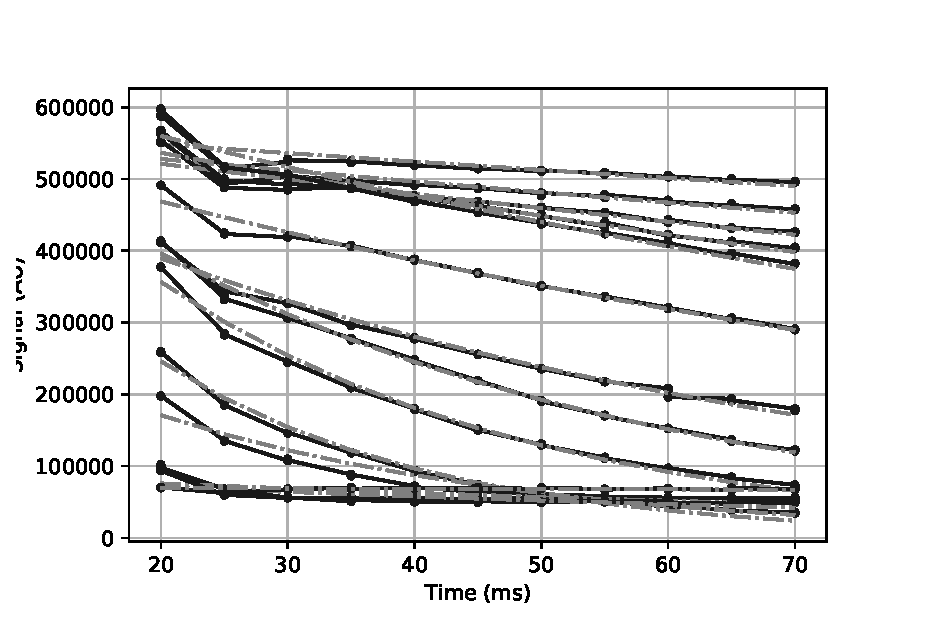
\includegraphics[width=1\textwidth]{T2_Mapping/Phantom/SE_raw.eps}
			\caption{}
			\label{fig:t2_phantom_se_raw}
		\end{subfigure}
		\hfill
		\begin{subfigure}[c]{0.47\textwidth}
			\centering
			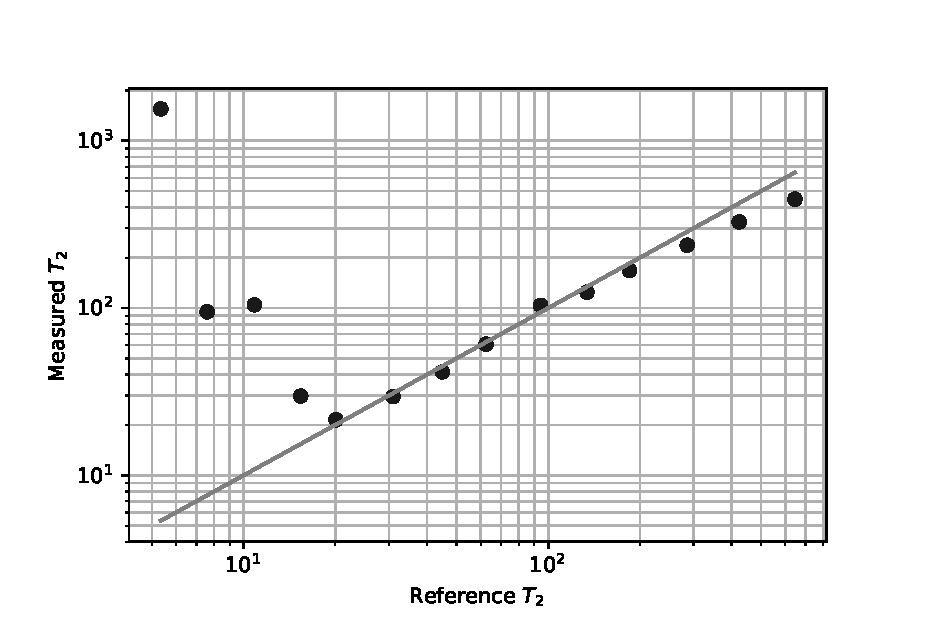
\includegraphics[width=1\textwidth]{T2_Mapping/Phantom/SE_mean.eps}
			\caption{}
			\label{fig:t2_phantom_se_mean}
		\end{subfigure}
	\end{subfigure}
	\vskip\baselineskip
	\begin{subfigure}[c]{0.9\textwidth}
		\centering
		\begin{subfigure}[c]{0.47\textwidth}
			\centering
			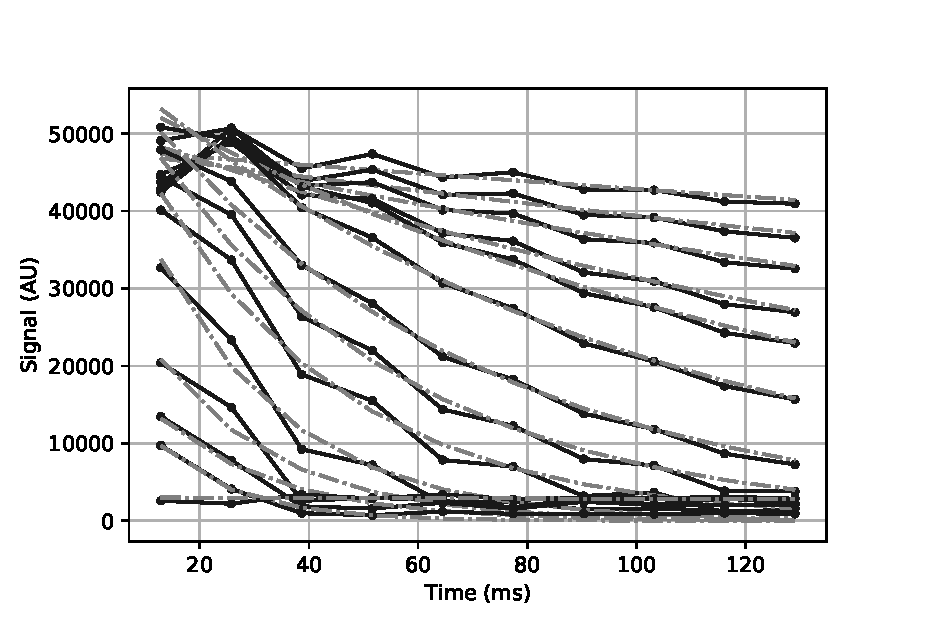
\includegraphics[width=1\textwidth]{T2_Mapping/Phantom/METSE_HR_raw.eps}
			\caption{}
			\label{fig:t2_phantom_metse_raw}
		\end{subfigure}
		\hfill
		\begin{subfigure}[c]{0.47\textwidth}
			\centering
			\includegraphics[width=1\textwidth]{T2_Mapping/Phantom/METSE_HR_mean.eps}
			\caption{}
			\label{fig:t2_phantom_metse_mean}
		\end{subfigure}
	\end{subfigure}
	\vskip\baselineskip
	\begin{subfigure}[c]{0.9\textwidth}
		\centering
		\begin{subfigure}[c]{0.47\textwidth}
			\centering
			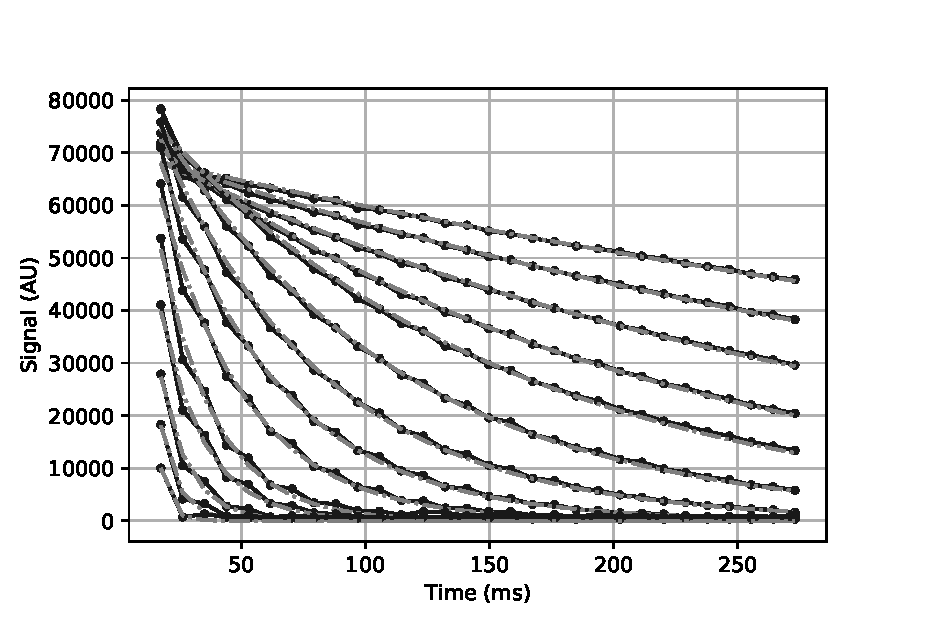
\includegraphics[width=1\textwidth]{T2_Mapping/Phantom/GraSE_HR_raw.eps}
			\caption{}
			\label{fig:t2_phantom_grase_raw}
		\end{subfigure}
		\hfill
		\begin{subfigure}[c]{0.47\textwidth}
			\centering
			\includegraphics[width=1\textwidth]{T2_Mapping/Phantom/GraSE_HR_mean.eps}
			\caption{}
			\label{fig:t2_phantom_grase_mean}
		\end{subfigure}
	\end{subfigure}
	\vskip\baselineskip
	\begin{subfigure}[c]{0.9\textwidth}
		\centering
		\begin{subfigure}[c]{0.47\textwidth}
			\centering
			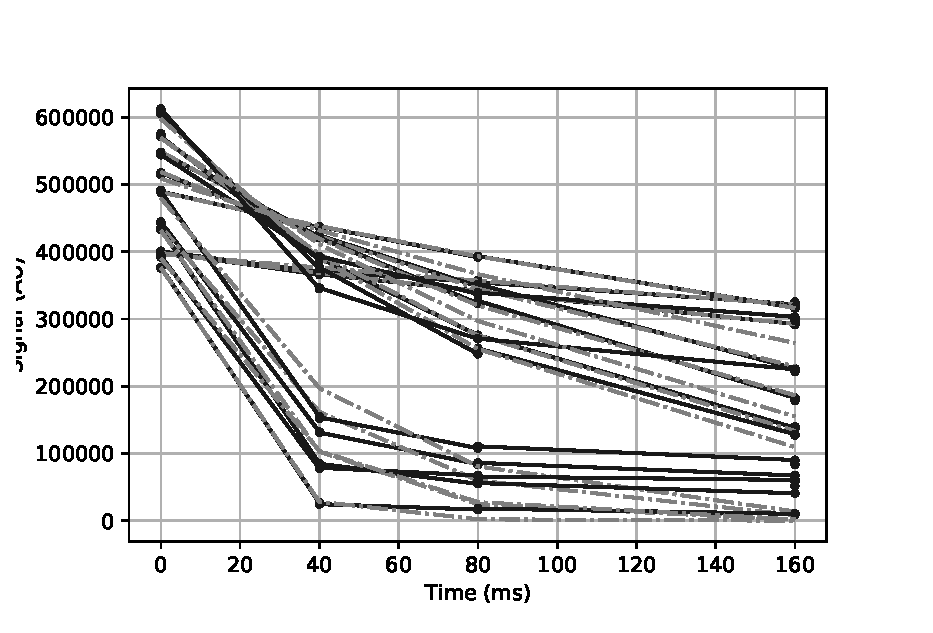
\includegraphics[width=1\textwidth]{T2_Mapping/Phantom/T2prep_raw.eps}
			\caption{}
			\label{fig:t2_phantom_t2prep_raw}
		\end{subfigure}
		\hfill
		\begin{subfigure}[c]{0.47\textwidth}
			\centering
			\includegraphics[width=1\textwidth]{T2_Mapping/Phantom/T2prep_mean.eps}
			\caption{}
			\label{fig:t2_phantom_t2prep_mean}
		\end{subfigure}
	\end{subfigure}
	\caption{Figures (\subref{fig:t2_phantom_se_raw}), (\subref{fig:t2_phantom_metse_raw}), (\subref{fig:t2_phantom_grase_raw}) and (\subref{fig:t2_phantom_t2prep_raw}) show the raw signal decay for each of the fourteen spheres and the fit decay. Figures (\subref{fig:t2_phantom_se_mean}), (\subref{fig:t2_phantom_metse_mean}), (\subref{fig:t2_phantom_grase_mean}) and (\subref{fig:t2_phantom_t2prep_mean}) show how the fit $T_2$ compares to the literature value. Figures (\subref{fig:t2_phantom_se_raw}) and (\subref{fig:t2_phantom_se_mean}) show the results from the \ac{SE}-\ac{EPI} method, (\subref{fig:t2_phantom_metse_raw}) and (\subref{fig:t2_phantom_metse_mean}) show the results form the \ac{ME-TSE} method, (\subref{fig:t2_phantom_grase_raw}) and (\subref{fig:t2_phantom_grase_mean}) show the results form the \ac{GraSE} method and (\subref{fig:t2_phantom_t2prep_raw}) and (\subref{fig:t2_phantom_t2prep_mean}) show the results from the $T_2$ prep method.} 
	\label{fig:t2_phantom}
\end{figure}

\subsection{Image Quality}

\subsection{In-Vivo}

$T_2$ maps using all four methods were collected on the same subject in the same scanning session to allow for a direct comparison of the in-vivo data. 

\begin{figure}[H]
	\centering
	\begin{subfigure}[c]{0.9\textwidth}
		\centering
		\begin{subfigure}[c]{0.47\textwidth}
			\centering
			\includegraphics[width=1\textwidth]{T2_Mapping/SE/SE_Raw_Echoes.eps}
			\caption{}
			\label{fig:t2_t2_se_raw}
		\end{subfigure}
		\hfill
		\begin{subfigure}[c]{0.47\textwidth}
			\centering
			\includegraphics[width=1\textwidth]{T2_Mapping/SE/SE_Map.eps}
			\caption{}
			\label{fig:t2_t2_se_map}
		\end{subfigure}
	\end{subfigure}
	\vskip\baselineskip
	\begin{subfigure}[c]{0.9\textwidth}
		\centering
		\includegraphics[width=1\textwidth]{T2_Mapping/SE/SE_Decay.eps}
		\caption{}
		\label{fig:t2_t2_se_decay}			
	\end{subfigure}
	\caption{(\subref{fig:t2_t2_se_raw}) The raw data used to generate the \ac{SE}-\ac{EPI} $T_2$ map.  (\subref{fig:t2_t2_se_map}) An example slice from the \ac{SE}-\ac{EPI} $T_2$ map. (\subref{fig:t2_t2_se_decay}) The signal decay for the renal cortex and medulla.} 
	\label{fig:t2_t2_se}
\end{figure}

The \ac{SE}-\ac{EPI} method (Figure \ref{fig:t2_t2_se}) generated maps with little blurring however there is also a lack of differentiation in $T_2$ between the renal cortex and medulla. The data collected at \ac{TE} of 20 ms appears to be artificially high and leads to a reduction in fit $T_2$. This sequence is the most susceptible of the methods to patient motion due to the acquisition method of a series per \ac{TE}, this increase in motion is clear when scrolling through \ac{TE}. 

\begin{figure}[H]
	\centering
	\begin{subfigure}[c]{0.9\textwidth}
		\centering
		\begin{subfigure}[c]{0.47\textwidth}
			\centering
			\includegraphics[width=1\textwidth]{T2_Mapping/ME/ME_Raw_Echoes.eps}
			\caption{}
			\label{fig:t2_t2_me_raw}
		\end{subfigure}
		\hfill
		\begin{subfigure}[c]{0.47\textwidth}
			\centering
			\includegraphics[width=1\textwidth]{T2_Mapping/ME/ME_Map.eps}
			\caption{}
			\label{fig:t2_t2_me_map}
		\end{subfigure}
	\end{subfigure}
	\vskip\baselineskip
	\begin{subfigure}[c]{0.9\textwidth}
		\centering
		\includegraphics[width=1\textwidth]{T2_Mapping/ME/ME_Decay.eps}
		\caption{}
		\label{fig:t2_t2_me_decay}			
	\end{subfigure}
	\caption{(\subref{fig:t2_t2_me_raw}) The raw data used to generate the \ac{ME-TSE} $T_2$ map.  (\subref{fig:t2_t2_me_map}) An example slice from the \ac{ME-TSE} $T_2$ map. (\subref{fig:t2_t2_me_decay}) The signal decay for the renal cortex and medulla.} 
	\label{fig:t2_t2_me}
\end{figure}

The map generated by the \ac{ME-TSE} method (Figure \ref{fig:t2_t2_me}) suffers from a large amount of blurring due to the relatively long echo train length. The number of echoes acquired is limited to the \ac{TSE} factor therefore to acquire ten echoes, a \ac{TSE} factor of ten needs to be used. This blurring leads to structures being obscured in the map and only a very small differentiation between cortex and medulla.

\begin{figure}[H]
	\centering
	\begin{subfigure}[c]{0.9\textwidth}
		\centering
		\begin{subfigure}[c]{0.47\textwidth}
			\centering
			\includegraphics[width=1\textwidth]{T2_Mapping/GraSE/GraSE_Raw_Echoes.eps}
			\caption{}
			\label{fig:t2_t2_grase_raw}
		\end{subfigure}
		\hfill
		\begin{subfigure}[c]{0.47\textwidth}
			\centering
			\includegraphics[width=1\textwidth]{T2_Mapping/GraSE/GraSE_Map.eps}
			\caption{}
			\label{fig:t2_t2_grase_map}
		\end{subfigure}
	\end{subfigure}
	\vskip\baselineskip
	\begin{subfigure}[c]{0.9\textwidth}
		\centering
		\includegraphics[width=1\textwidth]{T2_Mapping/GraSE/GraSE_Decay.eps}
		\caption{}
		\label{fig:t2_t2_grase_decay}			
	\end{subfigure}
	\caption{(\subref{fig:t2_t2_grase_raw}) The raw data used to generate the \ac{GraSE} $T_2$ map.  (\subref{fig:t2_t2_grase_map}) An example slice from the \ac{GraSE} $T_2$ map. (\subref{fig:t2_t2_grase_decay}) The signal decay for the renal cortex and medulla.}
	\label{fig:t2_t2_grase}
\end{figure}

Using the \ac{GraSE} method the data in Figure \ref{fig:t2_t2_grase} was collected. There is a clear difference between cortical and medullary $T_2$ and the data fits well to a $T_2$ decay (Figure \ref{fig:t2_t2_grase_decay}). The signal from the first echo in Figure \ref{fig:t2_t2_grase_decay} is too intense, this effect was even more pronounced when no startup echoes were used. For tissues with a longer $T_2$ using two startup echoes would be preferable however this makes measurements of tissues with a short $T_2$ more inaccurate, as such a compromise of a single startup echo was used. The short echo-spacing made possible by \ac{GraSE} means more \ac{TE} can be sampled and therefore leads to a more accurate fit.

\begin{figure}[H]
	\centering
	\begin{subfigure}[c]{0.9\textwidth}
		\centering
		\begin{subfigure}[c]{0.47\textwidth}
			\centering
			\includegraphics[width=1\textwidth]{T2_Mapping/T2prep/T2prep_Raw_Echoes.eps}
			\caption{}
			\label{fig:t2_t2_t2prep_raw}
		\end{subfigure}
		\hfill
		\begin{subfigure}[c]{0.47\textwidth}
			\centering
			\includegraphics[width=1\textwidth]{T2_Mapping/T2prep/T2prep_Map.eps}
			\caption{}
			\label{fig:t2_t2_t2prep_map}
		\end{subfigure}
	\end{subfigure}
	\vskip\baselineskip
	\begin{subfigure}[c]{0.9\textwidth}
		\centering
		\includegraphics[width=1\textwidth]{T2_Mapping/T2prep/T2prep_Decay.eps}
		\caption{}
		\label{fig:t2_t2_t2prep_decay}			
	\end{subfigure}
	\caption{(\subref{fig:t2_t2_t2prep_raw}) The mean data at each \ac{eTE} used to generate the $T_2$ preparation $T_2$ map.  (\subref{fig:t2_t2_t2prep_map}) An example slice from the $T_2$ preparation $T_2$ map. (\subref{fig:t2_t2_t2prep_decay}) The signal decay for the renal cortex and medulla.} 
	\label{fig:t2_t2_t2prep}
\end{figure}

The map made using the $T_2$ preparation method (Figure \ref{fig:t2_t2_t2prep}) suffers from noise in the raw data, this is despite there being three acquisitions at each \ac{eTE}. When comparing Figure \ref{fig:t2_t2_t2prep_map} to Figure \ref{fig:t2_t2_grase_map} it's possible to see that some of the areas of greater $T_2$ do match with the medulla, however the degree of noise in \ref{fig:t2_t2_t2prep_map} means it is un-usable on its own. The small number of \ac{eTE} collected means the uncertainty in the fit $T_2$ is higher for this method.

The two methods that have delivered the highest image quality, \ac{SE}-\ac{EPI} and \ac{GraSE}, produce substantially different values of $T_2$ in-vivo. Even when the data from the 20 ms volume is omitted from the \ac{SE}-\ac{EPI} fit, the $T_2$ is far lower. This is surprising give that when deployed on the phantom, this protocol delivered accurate results over the range of $T_2$ we see in the kidneys. This disparity is due to the additional confounding factors of diffusion and flow that are present in the body. These factors do not affect the \ac{GraSE} sequence to the same degree as the \ac{SE}-\ac{EPI} sequence.

\section{Discussion}
Of the methods explored, the \ac{GraSE} sequence produced the most accurate results on the phantom and superior image quality in-vivo, we will use this sequence in $T_2$ mapping going forward.

\section{Conclusion}

\section{Acknowledgements}

We are grateful for access to the University of Nottingham's Augusta high performance computing service.

\newpage
\section{References}
\defbibheading{bibliography}[\refname]{}
\printbibliography